\documentclass[10pt,a4paper]{article}
\usepackage[margin=1.3cm]{geometry}
\usepackage{amsmath, amssymb, amsthm}
\usepackage{tikz}
\usepackage{pgfplots}
\pgfplotsset{compat=1.18}
\usetikzlibrary{arrows.meta, decorations.pathreplacing, calc, patterns}
\usepackage{mdframed}
\usepackage{xcolor}
\usepackage{enumitem}
\usepackage{titlesec}
\usepackage{booktabs}
\usepackage{array}
\usepackage{multicol}
\usepackage{tcolorbox}
\tcbuselibrary{breakable, skins}
\usepackage{mathtools}
\usepackage{float}

%% ─── Colour Palette ──────────────────────────────────────────────────────────
\definecolor{headcolor}{RGB}{0,70,45}
\definecolor{darkgreen}{RGB}{0,110,65}
\definecolor{teal}{RGB}{0,128,128}
\definecolor{lightbg}{RGB}{237,255,246}
\definecolor{propbg}{RGB}{230,243,255}
\definecolor{exbg}{RGB}{255,249,232}
\definecolor{stepbg}{RGB}{235,242,255}
\definecolor{rampbg}{RGB}{248,235,255}
\definecolor{signumbg}{RGB}{255,241,238}
\definecolor{rectbg}{RGB}{240,255,241}
\definecolor{expbg}{RGB}{255,252,235}
\definecolor{notebg}{RGB}{255,250,220}
\definecolor{warningbg}{RGB}{255,240,240}
\definecolor{stepcolor}{RGB}{0,55,120}
\definecolor{rampcolor}{RGB}{100,0,110}
\definecolor{myorange}{RGB}{200,90,0}
\definecolor{mypurple}{RGB}{100,0,140}
\definecolor{myred}{RGB}{180,0,0}
\definecolor{myblue}{RGB}{0,60,180}

%% ─── Section Formatting ──────────────────────────────────────────────────────
\titleformat{\section}{\large\bfseries\color{headcolor}}{}{0em}{}[\color{darkgreen}\titlerule]
\titleformat{\subsection}{\normalsize\bfseries\color{darkgreen}}{}{0em}{}
\titleformat{\subsubsection}{\small\bfseries\color{teal}}{}{0em}{}
\titlespacing{\section}{0pt}{9pt}{4pt}
\titlespacing{\subsection}{0pt}{6pt}{2pt}
\titlespacing{\subsubsection}{0pt}{4pt}{1pt}

%% ─── Box Environments (tcolorbox) ─────────────────────────────────────────────
\newtcolorbox{defbox}[1][]{breakable,
  colback=lightbg, colframe=darkgreen, arc=3pt,
  boxrule=0.8pt, left=5pt, right=5pt, top=4pt, bottom=4pt,
  title={\small\bfseries\color{darkgreen}Definition}, #1}
\newtcolorbox{propbox}[1][]{breakable,
  colback=propbg, colframe=teal, arc=3pt,
  boxrule=0.8pt, left=5pt, right=5pt, top=4pt, bottom=4pt,
  title={\small\bfseries\color{teal}Properties}, #1}
\newtcolorbox{exbox}[1][]{breakable,
  colback=exbg, colframe=myorange, arc=3pt,
  boxrule=0.8pt, left=5pt, right=5pt, top=4pt, bottom=4pt,
  title={\small\bfseries\color{myorange}Solved Examples}, #1}
\newtcolorbox{notebox}[1][]{breakable,
  colback=notebg, colframe=myorange!70!black, arc=3pt,
  boxrule=0.8pt, left=5pt, right=5pt, top=3pt, bottom=3pt,
  title={\small\bfseries\color{myorange!80!black}Key Note}, #1}
\newtcolorbox{derivbox}[1][]{breakable,
  colback=rampbg, colframe=rampcolor, arc=3pt,
  boxrule=0.8pt, left=5pt, right=5pt, top=4pt, bottom=4pt,
  title={\small\bfseries\color{rampcolor}Derivation}, #1}
\newtcolorbox{chainbox}[1][]{breakable,
  colback=stepbg, colframe=stepcolor, arc=3pt,
  boxrule=0.8pt, left=5pt, right=5pt, top=4pt, bottom=4pt,
  title={\small\bfseries\color{stepcolor}Signal Chain}, #1}

%% ─── Misc ─────────────────────────────────────────────────────────────────────
\setlength{\parindent}{0pt}
\setlength{\parskip}{2pt}
\setlist[itemize]{noitemsep, topsep=1pt, leftmargin=14pt}
\setlist[enumerate]{noitemsep, topsep=1pt, leftmargin=14pt}

\newcommand{\DD}{\dfrac{d}{dt}}
\newcommand{\Int}{\displaystyle\int_{-\infty}^{\infty}}
\newcommand{\Intt}{\displaystyle\int_{-\infty}^{t}}

\begin{document}

%% ══════════════════════════════════════════════════════════════════════════════
%%  TITLE
%% ══════════════════════════════════════════════════════════════════════════════
\begin{center}
  {\LARGE\bfseries\color{headcolor} Signals \& Systems --- Comprehensive Reference}\\[4pt]
  {\normalsize\color{darkgreen}
    Unit Impulse $\cdot$ Sampling Property $\cdot$ Unit Step $\cdot$ Impulse--Step Relation
    $\cdot$ Unit Ramp $\cdot$ Unit Parabolic $\cdot$ Signum $\cdot$ Rectangular
    $\cdot$ Triangular $\cdot$ Sinc $\cdot$ Exponential Signals}\\[2pt]
  {\small\color{gray} EC002 --- Complete Study Notes with Derivations \& Worked Problems}
\end{center}
\vspace{2pt}
{\color{darkgreen}\rule{\linewidth}{1.5pt}}
\vspace{4pt}

%% ══════════════════════════════════════════════════════════════════════════════
\section{1.\ Unit Impulse Signal (Dirac Delta Function)}
%% ══════════════════════════════════════════════════════════════════════════════

\begin{defbox}
The \textbf{unit impulse signal} $\delta(t)$, also called the \textbf{Dirac delta function}, is defined as:
\[
  \delta(t) = \begin{cases} \infty & t = 0 \\ 0 & t \neq 0 \end{cases}
  \qquad \text{subject to the constraint:} \qquad
  \Int \delta(t)\,dt = 1
\]
It is not a function in the classical sense --- it is a \emph{distribution} (or \emph{generalized function}).
Its \textbf{area is always 1}, regardless of how compressed it is.
A weighted impulse $A_0\,\delta(t)$ has area $A_0$ and is drawn as an arrow of height $A_0$.
\end{defbox}

\subsection*{Graphical Representation}

\begin{center}
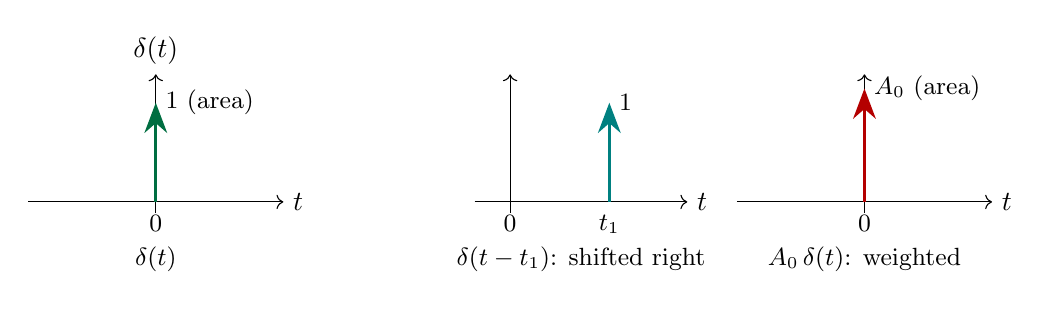
\begin{tikzpicture}[scale=0.9]
  % Left: basic delta(t)
  \begin{scope}[xshift=0cm]
    \draw[->] (-1.8,0) -- (1.8,0) node[right] {$t$};
    \draw[->] (0,-0.15) -- (0,1.8) node[above] {$\delta(t)$};
    \draw[-{Stealth[scale=1.3]}, very thick, darkgreen] (0,0) -- (0,1.4);
    \node[below, font=\small] at (0,-0.05) {$0$};
    \node[right, font=\small] at (0,1.4) {$1$ (area)};
    \node[font=\small, below] at (0,-0.5) {$\delta(t)$};
  \end{scope}
  % Middle: delta(t-t1)
  \begin{scope}[xshift=5cm]
    \draw[->] (-0.5,0) -- (2.5,0) node[right] {$t$};
    \draw[->] (0,-0.15) -- (0,1.8) node[above] {};
    \draw[-{Stealth[scale=1.3]}, very thick, teal] (1.4,0) -- (1.4,1.4);
    \node[below, font=\small] at (0,-0.05) {$0$};
    \node[below, font=\small] at (1.4,-0.05) {$t_1$};
    \node[right, font=\small] at (1.4,1.4) {$1$};
    \node[font=\small, below] at (1,-0.5) {$\delta(t-t_1)$: shifted right};
  \end{scope}
  % Right: A0*delta(t)
  \begin{scope}[xshift=10cm]
    \draw[->] (-1.8,0) -- (1.8,0) node[right] {$t$};
    \draw[->] (0,-0.15) -- (0,1.8) node[above] {};
    \draw[-{Stealth[scale=1.3]}, very thick, myred] (0,0) -- (0,1.6);
    \node[below, font=\small] at (0,-0.05) {$0$};
    \node[right, font=\small] at (0,1.6) {$A_0$ (area)};
    \node[font=\small, below] at (0,-0.5) {$A_0\,\delta(t)$: weighted};
  \end{scope}
\end{tikzpicture}
\end{center}

\subsection*{Derivation via Rectangular Pulse Limit}

\begin{derivbox}
Consider a rectangular pulse $x_\varepsilon(t)$ of width $\varepsilon$ and height $\frac{1}{\varepsilon}$:
\[
  x_\varepsilon(t) = \begin{cases} \frac{1}{\varepsilon} & -\frac{\varepsilon}{2} < t < \frac{\varepsilon}{2} \\ 0 & \text{otherwise} \end{cases}
  \qquad \Rightarrow \qquad \text{Area} = \varepsilon \times \frac{1}{\varepsilon} = 1 \quad \forall\,\varepsilon
\]
As $\varepsilon \to 0$: width $\to 0$, height $\to \infty$, but area remains exactly $1$.
Therefore: $\delta(t) = \displaystyle\lim_{\varepsilon \to 0} x_\varepsilon(t)$.

\smallskip
This can also be approached via a \textbf{Gaussian}: $\delta(t) = \lim_{\sigma\to0} \frac{1}{\sigma\sqrt{2\pi}}e^{-t^2/2\sigma^2}$, or a \textbf{sinc sequence}: $\delta(t)=\lim_{W\to\infty}\frac{\sin(Wt)}{\pi t}$.
\end{derivbox}

\begin{center}
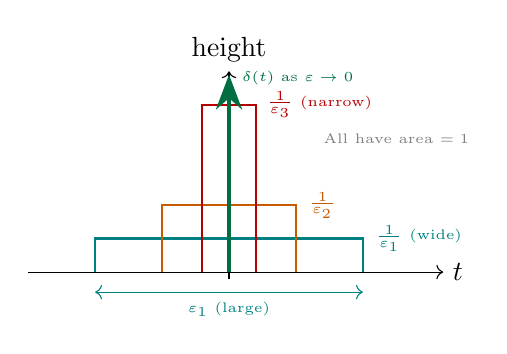
\begin{tikzpicture}[scale=0.85]
  \draw[->] (-3,0) -- (3.2,0) node[right] {$t$};
  \draw[->] (0,-0.1) -- (0,3.0) node[above] {height};
  % Wide pulse
  \draw[teal, thick] (-2,0)--(-2,0.5)--(2,0.5)--(2,0);
  \node[teal, font=\tiny, right] at (2.05,0.5) {$\frac{1}{\varepsilon_1}$ (wide)};
  \draw[<->, teal, thin] (-2,-0.3)--(2,-0.3) node[midway,below,font=\tiny]{$\varepsilon_1$ (large)};
  % Narrower pulse
  \draw[myorange, thick] (-1,0)--(-1,1.0)--(1,1.0)--(1,0);
  \node[myorange, font=\tiny, right] at (1.05,1.0) {$\frac{1}{\varepsilon_2}$};
  % Narrow pulse
  \draw[myred, thick] (-0.4,0)--(-0.4,2.5)--(0.4,2.5)--(0.4,0);
  \node[myred, font=\tiny, right] at (0.42,2.5) {$\frac{1}{\varepsilon_3}$ (narrow)};
  % Arrow showing limit
  \draw[-{Stealth[scale=1.5]}, darkgreen, very thick] (0,0) -- (0,2.95);
  \node[darkgreen, right, font=\tiny] at (0.05,2.9) {$\delta(t)$ as $\varepsilon\to0$};
  \node[font=\tiny, gray] at (2.5,2.0) {All have area $=1$};
\end{tikzpicture}
\end{center}

\subsection*{Complete Properties of the Impulse Signal}

\begin{propbox}
\textbf{P1 --- Unit Area (Normalization):}
\[
  \Int \delta(t)\,dt = 1
\]
This is the defining property. The total ``weight'' of the impulse is always 1.

\medskip
\textbf{P2 --- Strength / Weight:}
If $y(t) = A_0\,\delta(t)$, then $\displaystyle\Int y(t)\,dt = A_0$.
The number $A_0$ is called the \emph{strength} (weight) of the impulse, shown as a number beside the arrow.

\medskip
\textbf{P3 --- Integration gives Unit Step:}
\[
  \Intt \delta(\tau)\,d\tau = u(t) \qquad \text{and} \qquad \Intt A_0\,\delta(\tau)\,d\tau = A_0\,u(t)
\]
Conversely, $\dfrac{d}{dt}u(t) = \delta(t)$.

\medskip
\textbf{P4 --- Even Symmetry:}
\[
  \delta(-t) = \delta(t) \qquad (\text{impulse is an \textbf{even} function})
\]
Proof: For any test function $\phi$, $\int \delta(-t)\phi(t)\,dt = \int \delta(\tau)\phi(-\tau)\,d\tau = \phi(0) = \int\delta(t)\phi(t)\,dt$.

\medskip
\textbf{P5 --- Energy \& Power Classification:}
\[
  E = \Int |\delta(t)|^2\,dt = \infty, \quad P = \infty \qquad \Rightarrow \quad \textbf{NENP signal}
\]
(Neither Energy nor Power signal because both $E$ and $P$ are infinite.)

\medskip
\textbf{P6 --- Time Shifting:}
\[
  \delta(t - t_0) \text{ is an impulse located at } t = t_0
\]

\medskip
\textbf{P7 --- Time Scaling:}
\[
  \delta(at) = \frac{1}{|a|}\delta(t), \qquad a \neq 0
\]
\textit{Proof:} Let $\tau = at$, $d\tau = a\,dt$. Then $\int\delta(at)\phi(t)\,dt = \frac{1}{|a|}\int\delta(\tau)\phi(\tau/a)\,d\tau = \frac{1}{|a|}\phi(0)$.

\quad\textit{Example i:} $\delta(-2t) = \tfrac{1}{2}\delta(t)$ \hfill (scaling by $a=-2$)

\quad\textit{Example ii:} $\delta(-2t+3) = \delta\bigl[-2\bigl(t-\tfrac{3}{2}\bigr)\bigr] = \tfrac{1}{2}\delta\bigl(t-\tfrac{3}{2}\bigr)$

\medskip
\textbf{P8 --- Multiplication Property:}
\[
  x(t)\cdot\delta(t - t_0) = x(t_0)\cdot\delta(t - t_0)
\]
Since $\delta(t-t_0)=0$ for $t\neq t_0$, $x(t)$ is effectively frozen at $t=t_0$.

\quad\textit{Example i:} $2t^2\cdot\delta(t-3) = 2(3)^2\,\delta(t-3) = 18\,\delta(t-3)$

\quad\textit{Example ii:} $\cos4t\cdot\delta(2t-\pi)$: first write $\delta(2t-\pi)=\tfrac{1}{2}\delta(t-\tfrac{\pi}{2})$, so the product $= \cos(2\pi)\cdot\tfrac{1}{2}\delta(t-\tfrac{\pi}{2}) = \tfrac{1}{2}\delta(t-\tfrac{\pi}{2})$.

\medskip
\textbf{P9 --- Sifting (Sampling) Property:}
\[
  \Int x(t)\,\delta(t - t_0)\,dt = x(t_0)
\]
The impulse ``sifts out'' (samples) the value of $x$ exactly at $t = t_0$.
\begin{itemize}
  \item If $t_0$ is \emph{outside} the limits of integration $\Rightarrow$ result $= 0$
  \item If $t_0$ is \emph{inside} the limits of integration $\Rightarrow$ result $= x(t_0)$
\end{itemize}

\medskip
\textbf{P10 --- Derivative Property ($n$th order):}
\[
  \Int x(t)\,\frac{d^n}{dt^n}\delta(t - t_0)\,dt = (-1)^n \left.\frac{d^n x}{dt^n}\right|_{t=t_0}
\]
(valid when $x(t)$ and its derivatives are finite at $\pm\infty$)

\quad\textit{Example:} $\Int \cos\pi t \cdot \dfrac{d^2\delta(t-1)}{dt^2}\,dt = (-1)^2 \dfrac{d^2}{dt^2}\cos\pi t\Big|_{t=1} = (-\pi^2\cos\pi)\big|_1 = \pi^2$

\medskip
\textbf{P11 --- Doublet (Derivative of Impulse):}
\[
  \delta'(t) = \frac{d\,\delta(t)}{dt} \quad \text{called the \textbf{doublet} or dipole function --- it is an \textbf{odd} signal}
\]
$\Int \delta'(t)\,dt = 0$ (zero total area). Used in circuit analysis with initial conditions.
\end{propbox}

\subsection*{Summary Table of Impulse Properties}

\begin{center}
{\small
\begin{tabular}{@{}c l l@{}}
\toprule
\textbf{\#} & \textbf{Property} & \textbf{Formula / Statement}\\
\midrule
1 & Unit Area & $\Int\delta(t)\,dt=1$ \\[4pt]
2 & Strength & $\Int A_0\delta(t)\,dt=A_0$ \\[4pt]
3 & Integration & $\Intt\delta(\tau)\,d\tau=u(t)$; \quad $\tfrac{d}{dt}u(t)=\delta(t)$ \\[4pt]
4 & Even symmetry & $\delta(-t)=\delta(t)$ \\[2pt]
5 & Energy/Power & NENP: $E=\infty,\;P=\infty$ \\[2pt]
6 & Time shift & $\delta(t-t_0)$: impulse at $t=t_0$ \\[2pt]
7 & Time scale & $\delta(at)=\tfrac{1}{|a|}\delta(t)$ \\[4pt]
8 & Multiplication & $x(t)\delta(t-t_0)=x(t_0)\delta(t-t_0)$ \\[4pt]
9 & Sifting integral & $\Int x(t)\delta(t-t_0)\,dt=x(t_0)$ \\[4pt]
10 & $n$th derivative & $\Int x(t)\frac{d^n\delta}{dt^n}\,dt=(-1)^n x^{(n)}(t_0)$ \\[4pt]
11 & Doublet & $\tfrac{d}{dt}\delta(t)$: odd signal, zero area \\[2pt]
\bottomrule
\end{tabular}
}
\end{center}

\subsection*{Fully Worked Problems --- Unit Impulse}

\begin{exbox}
\textbf{Problem 1:} Evaluate $I=\displaystyle\int_{-5}^{4}\delta(t-5)\,dt$

\textbf{Solution:} The impulse fires at $t_0=5$. Check: is $5\in[-5,4]$? \textbf{No} ($5>4$). Therefore $I=\boxed{0}$.

\medskip
\textbf{Problem 2:} Evaluate $I=\displaystyle\int_{-5}^{4}\delta(t-2)\,dt$

\textbf{Solution:} The impulse fires at $t_0=2$. Check: is $2\in[-5,4]$? \textbf{Yes}. Therefore $I=\boxed{1}$.

\medskip
\textbf{Problem 3:} Simplify $x(t)=\sin t\cdot\delta(2t-\pi)$

\textbf{Step 1:} Apply time-scaling to $\delta(2t-\pi)=\delta\bigl[2(t-\tfrac{\pi}{2})\bigr]=\tfrac{1}{2}\delta(t-\tfrac{\pi}{2})$

\textbf{Step 2:} Apply multiplication property: $x(t)=\sin\!\bigl(\tfrac{\pi}{2}\bigr)\cdot\tfrac{1}{2}\delta\!\bigl(t-\tfrac{\pi}{2}\bigr)=1\cdot\tfrac{1}{2}\delta\!\bigl(t-\tfrac{\pi}{2}\bigr)=\boxed{\dfrac{1}{2}\delta\!\bigl(t-\tfrac{\pi}{2}\bigr)}$

\medskip
\textbf{Problem 4:} Evaluate $I=\displaystyle\Int e^{-2t}\,\delta(-2t+1)\,dt$

\textbf{Step 1:} $\delta(-2t+1)=\delta\bigl[-2(t-\tfrac{1}{2})\bigr]=\tfrac{1}{2}\delta(t-\tfrac{1}{2})$

\textbf{Step 2:} Sifting: $I=\tfrac{1}{2}\cdot e^{-2\cdot(1/2)}=\tfrac{1}{2}e^{-1}=\boxed{\dfrac{1}{2e}}$

\medskip
\textbf{Problem 5 (Composite):} $I=\displaystyle\Int\!\bigl[\cos\pi t\cdot\delta(t-2)+3\delta(t+1)+\sin\pi t\cdot\delta(2t-1)\bigr]dt$

\textbf{Part 1:} $I_1 = \cos(2\pi)=1$

\textbf{Part 2:} $I_2 = 3\cdot\Int\delta(t+1)\,dt=3\cdot 1=3$

\textbf{Part 3:} $\delta(2t-1)=\tfrac{1}{2}\delta(t-\tfrac{1}{2})$, so $I_3=\tfrac{1}{2}\sin(\tfrac{\pi}{2})=\tfrac{1}{2}$

$\therefore\quad I = 1+3+0.5 = \boxed{4.5}$

\medskip
\textbf{Problem 6 [GATE 2016]:} $I=\displaystyle\Int e^{-t}\,\delta(2t-2)\,dt$

$\delta(2t-2)=\delta\bigl[2(t-1)\bigr]=\tfrac{1}{2}\delta(t-1)$

$I=\tfrac{1}{2}e^{-1}=\boxed{\dfrac{1}{2e}}\approx 0.184$ \quad\textbf{(Answer: option a)}

\medskip
\textbf{Problem 7 (Boundary check):}

$I=\displaystyle\int_{-2}^{2}2t^2\delta(t-4)\,dt$: $t_0=4\notin[-2,2]$ $\Rightarrow$ $I=\boxed{0}$

$I=\displaystyle\int_{-10}^{10}2t^2\delta(t-4)\,dt$: $t_0=4\in[-10,10]$ $\Rightarrow$ $I=2(4)^2=\boxed{32}$

\medskip
\textbf{Problem 8 (Derivative property):} $I=\displaystyle\Int\cos\pi t\cdot\frac{d^2\delta(t-1)}{dt^2}\,dt$

Using P10 with $n=2$, $t_0=1$: $I=(-1)^2\dfrac{d^2}{dt^2}[\cos\pi t]\Big|_{t=1}$

$\dfrac{d^2}{dt^2}[\cos\pi t]=-\pi^2\cos\pi t$. At $t=1$: $-\pi^2\cos\pi = -\pi^2(-1) = \pi^2$. $\Rightarrow I=\boxed{\pi^2}$
\end{exbox}

%% ══════════════════════════════════════════════════════════════════════════════
\section{2.\ Sampling (Sifting) Property of the Unit Impulse}
%% ══════════════════════════════════════════════════════════════════════════════

\begin{defbox}
The \textbf{sampling property} states: when any signal $x(t)$ is multiplied by a shifted impulse $\delta(t-\tau)$, the result is a new signal that is zero everywhere except at $t=\tau$, where it takes the value $x(\tau)$:
\[
  x(t)\cdot\delta(t-\tau) = x(\tau)\cdot\delta(t-\tau)
\]
When this product is integrated, it ``sifts out'' the single sample $x(\tau)$:
\[
  \Int x(t)\cdot\delta(t-\tau)\,dt = x(\tau)
\]
This is why this is also called the \textbf{sifting property} --- the impulse acts like a sieve, retaining only the value at $t=\tau$ and discarding all others.
\end{defbox}

\subsection*{Visual Interpretation}

\begin{center}
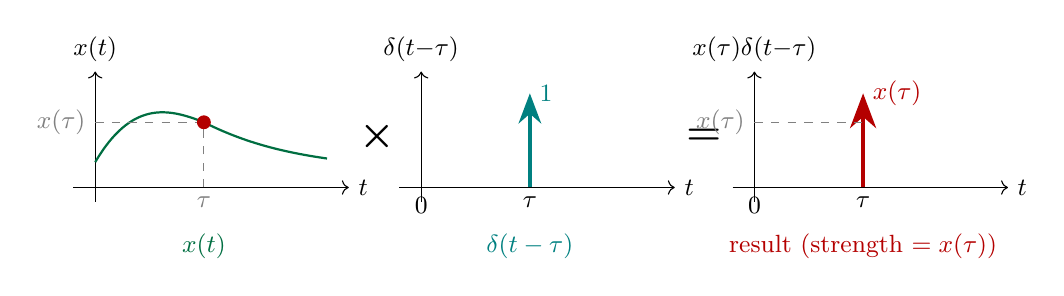
\begin{tikzpicture}[scale=0.92]
  % Panel 1: x(t)
  \begin{scope}[xshift=0cm]
    \draw[->](-0.3,0)--(3.5,0) node[right]{\small$t$};
    \draw[->](0,-0.2)--(0,1.6) node[above]{\small$x(t)$};
    \draw[darkgreen,thick,smooth] (0,0.35) ..controls(0.5,1.2) and (1.0,1.1).. (1.5,0.9)
      ..controls (2.0,0.65) and (2.5,0.5).. (3.2,0.4);
    \draw[dashed,gray](1.5,0) node[below]{\small$\tau$}--(1.5,0.9);
    \draw[dashed,gray](0,0.9) node[left]{\small$x(\tau)$}--(1.5,0.9);
    \filldraw[myred](1.5,0.9) circle(2.5pt);
    \node[below,font=\small,darkgreen] at (1.5,-0.5){$x(t)$};
  \end{scope}
  % Times sign
  \node at(3.9,0.7){\Large$\boldsymbol{\times}$};
  % Panel 2: delta(t-tau)
  \begin{scope}[xshift=4.5cm]
    \draw[->](-0.3,0)--(3.5,0) node[right]{\small$t$};
    \draw[->](0,-0.2)--(0,1.6) node[above]{\small$\delta(t{-}\tau)$};
    \draw[-{Stealth[scale=1.3]},very thick,teal](1.5,0)--(1.5,1.3);
    \node[below,font=\small] at(0,0){$0$};
    \node[below,font=\small] at(1.5,0){$\tau$};
    \node[right,font=\small,teal] at(1.5,1.3){$1$};
    \node[below,font=\small,teal] at (1.5,-0.5){$\delta(t-\tau)$};
  \end{scope}
  % Equals sign
  \node at(8.4,0.7){\Large$\boldsymbol{=}$};
  % Panel 3: x(tau)*delta(t-tau)
  \begin{scope}[xshift=9.1cm]
    \draw[->](-0.3,0)--(3.5,0) node[right]{\small$t$};
    \draw[->](0,-0.2)--(0,1.6) node[above]{\small$x(\tau)\delta(t{-}\tau)$};
    \draw[-{Stealth[scale=1.5]},very thick,myred](1.5,0)--(1.5,1.3);
    \node[below,font=\small] at(0,0){$0$};
    \node[below,font=\small] at(1.5,0){$\tau$};
    \node[right,font=\small,myred] at(1.5,1.3){$x(\tau)$};
    \draw[dashed,gray] (0,0.9)node[left,font=\small]{$x(\tau)$} -- (1.5,0.9);
    \node[below,font=\small,myred] at (1.5,-0.5){result (strength $=x(\tau)$)};
  \end{scope}
\end{tikzpicture}
\end{center}

\begin{propbox}
\textbf{Formal statement:} For any signal $x(t)$ continuous at $t=\tau$:
\[
  \Int x(t)\,\delta(t-\tau)\,dt = x(\tau)
\]
\textbf{Partial-interval version:}
\[
  \int_a^b x(t)\,\delta(t-\tau)\,dt = \begin{cases} x(\tau) & a < \tau < b \\ 0 & \tau < a \text{ or } \tau > b \end{cases}
\]
\textbf{Physical interpretation:} The impulse is like an ``ideal sampler'' --- it extracts an instantaneous snapshot of $x(t)$ at the moment $t=\tau$.
In digital signal processing, the sampling of a continuous signal is modelled by a train of impulses: $x_s(t)=x(t)\cdot\sum_{n=-\infty}^{\infty}\delta(t-nT_s)$, where $T_s$ is the sampling period.
\end{propbox}

\begin{exbox}
\textbf{Example 1:} $\displaystyle\Int (t^2+2t+1)\,\delta(t-3)\,dt = (9+6+1) = \boxed{16}$

\textbf{Example 2:} $\displaystyle\int_0^{10} e^{-2t}\,\delta(t-1)\,dt = e^{-2}$ \quad (since $t_0=1\in(0,10)$) $=\boxed{e^{-2}}$

\textbf{Example 3:} $\displaystyle\Int \cos(\omega t)\,\delta(t-\tfrac{\pi}{2\omega})\,dt = \cos\!\bigl(\omega\cdot\tfrac{\pi}{2\omega}\bigr)=\cos\tfrac{\pi}{2}=\boxed{0}$
\end{exbox}

%% ══════════════════════════════════════════════════════════════════════════════
\section{3.\ Unit Step Signal (Heaviside Step Function)}
%% ══════════════════════════════════════════════════════════════════════════════

\begin{defbox}
The \textbf{unit step signal} (also called the \textbf{Heaviside function}) is defined as:
\[
  u(t) = \begin{cases} 0 & t < 0 \\ 1 & t \geq 0 \end{cases}
\]
It switches from 0 to 1 at $t=0$. The value at $t=0$ is sometimes left undefined (in the distributional sense) or taken as $\tfrac{1}{2}$ (using the Gibbs/average convention).

A shifted unit step $u(t-t_0)$ switches ON at $t=t_0$.
\end{defbox}

\subsection*{Graphical Representation and Variants}

\begin{center}
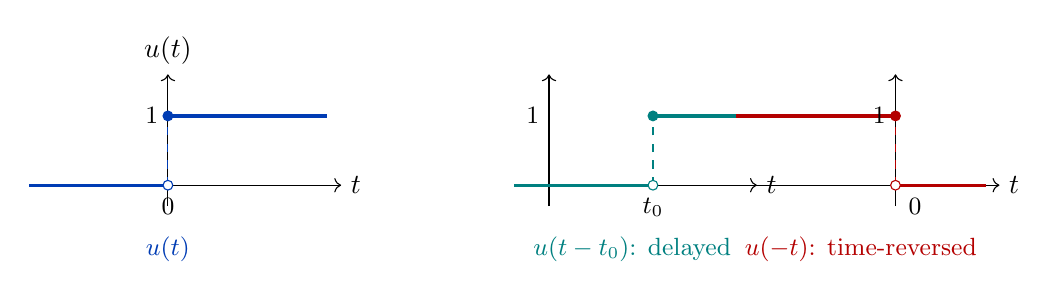
\begin{tikzpicture}[scale=0.88]
  % u(t)
  \begin{scope}[xshift=0cm]
    \draw[->](-2,0)--(2.5,0) node[right]{$t$};
    \draw[->](0,-0.3)--(0,1.6) node[above]{$u(t)$};
    \draw[myblue,very thick](-2,0)--(0,0);
    \draw[myblue,very thick](0,1)--(2.3,1);
    \draw[myblue,dashed](0,0)--(0,1);
    \filldraw[myblue](0,1) circle(2pt);
    \filldraw[white,draw=myblue](0,0) circle(2pt);
    \node[left,font=\small] at(0,1){$1$};
    \node[below,font=\small] at(0,-0.05){$0$};
    \node[below,font=\small,myblue] at (0,-0.6){$u(t)$};
  \end{scope}
  % u(t-t0)
  \begin{scope}[xshift=5.5cm]
    \draw[->](-0.5,0)--(3.0,0) node[right]{$t$};
    \draw[->](0,-0.3)--(0,1.6) node[above]{};
    \draw[teal,very thick](-0.5,0)--(1.5,0);
    \draw[teal,very thick](1.5,1)--(2.8,1);
    \draw[teal,dashed](1.5,0)--(1.5,1);
    \filldraw[teal](1.5,1) circle(2pt);
    \filldraw[white,draw=teal](1.5,0) circle(2pt);
    \node[below,font=\small] at(1.5,-0.05){$t_0$};
    \node[left,font=\small] at(0,1){$1$};
    \node[below,font=\small,teal] at (1.2,-0.6){$u(t-t_0)$: delayed};
  \end{scope}
  % u(-t)
  \begin{scope}[xshift=10.5cm]
    \draw[->](-2.5,0)--(1.5,0) node[right]{$t$};
    \draw[->](0,-0.3)--(0,1.6) node[above]{};
    \draw[myred,very thick](-2.3,1)--(0,1);
    \draw[myred,very thick](0,0)--(1.3,0);
    \draw[myred,dashed](0,0)--(0,1);
    \filldraw[myred](0,1) circle(2pt);
    \filldraw[white,draw=myred](0,0) circle(2pt);
    \node[left,font=\small] at(0,1){$1$};
    \node[below right,font=\small] at(0.05,-0.05){$0$};
    \node[below,font=\small,myred] at (-0.5,-0.6){$u(-t)$: time-reversed};
  \end{scope}
\end{tikzpicture}
\end{center}

\subsection*{Properties of the Unit Step Signal}

\begin{propbox}
\textbf{P1 --- Relation to $u(t)+u(-t)$:}
\[
  u(t)+u(-t)=\begin{cases}1+0=1 & t>0 \\ 0+1=1 & t<0 \\ 1+1=2 & t=0\end{cases}
\]
The sum equals 1 everywhere except at $t=0$ where it equals 2.

\medskip
\textbf{P2 --- Power Calculation:}
\[
  P = \lim_{T\to\infty}\frac{1}{2T}\int_{-T}^{T}|u(t)|^2\,dt
    = \lim_{T\to\infty}\frac{1}{2T}\Bigl[\underbrace{\int_{-T}^{0}0\,dt}_{=0}+\int_{0}^{T}1^2\,dt\Bigr]
    = \lim_{T\to\infty}\frac{T}{2T} = \frac{1}{2}
\]
$E = \infty$ (energy over $[0,\infty)$ diverges), $P = \tfrac{1}{2}$ (finite) $\Rightarrow$ \textbf{Power signal}. \quad $P_{\rm rms} = \sqrt{P} = \dfrac{1}{\sqrt{2}}$.

\medskip
\textbf{P3 --- Symmetry:}
$u(t) \neq u(-t)$ and $u(t) \neq -u(-t)$ $\Rightarrow$ \textbf{neither even nor odd} (asymmetric)

\medskip
\textbf{P4 --- Building block for other signals:}\\
Any piecewise constant signal can be expressed using shifted and weighted steps.
\begin{itemize}
  \item Rectangular pulse: $\mathrm{rect}(t) = u(t+\tfrac{a}{2}) - u(t-\tfrac{a}{2})$
  \item Gating a signal $x(t)$ on $[a,b]$: $x(t)\bigl[u(t-a)-u(t-b)\bigr]$
\end{itemize}

\medskip
\textbf{P5 --- Derivative and Integral:}
\[
  \frac{d}{dt}u(t) = \delta(t) \qquad\qquad \Intt u(\tau)\,d\tau = t\,u(t) = r(t)
\]

\medskip
\textbf{P6 --- Gibbs Phenomenon at discontinuity:}
For the Fourier series of $u(t)$, at the jump discontinuity at $t=0$, the series converges to the \textbf{average} of the left and right limits: $\dfrac{0+1}{2}=\dfrac{1}{2}$.
\end{propbox}

%% ══════════════════════════════════════════════════════════════════════════════
\section{4.\ Relation Between Impulse and Step Signal}
%% ══════════════════════════════════════════════════════════════════════════════

\begin{defbox}
The impulse and step are \textbf{integral--derivative pairs}:
\[
  \boxed{\int_{-\infty}^{t}\delta(\tau)\,d\tau = u(t)}
  \qquad\qquad
  \boxed{\frac{d\,u(t)}{dt} = \delta(t)}
\]
\end{defbox}

\subsection*{Rigorous Derivation via Slope Approximation}

\begin{derivbox}
Define a smooth approximation to $u(t)$ using a linear ramp:
\[
  u_\Delta(t) = \begin{cases} 0 & t < 0 \\ t/\Delta & 0 \leq t \leq \Delta \\ 1 & t > \Delta \end{cases}
\]
Its derivative is:
\[
  \frac{d\,u_\Delta(t)}{dt} = \begin{cases} 1/\Delta & 0 < t < \Delta \\ 0 & \text{elsewhere} \end{cases}
\]
This derivative is a rectangular pulse of height $\tfrac{1}{\Delta}$ and width $\Delta$, so area $= 1$.
As $\Delta\to0$: $u_\Delta(t)\to u(t)$ and $\tfrac{d\,u_\Delta}{dt}\to\delta(t)$.

\begin{center}
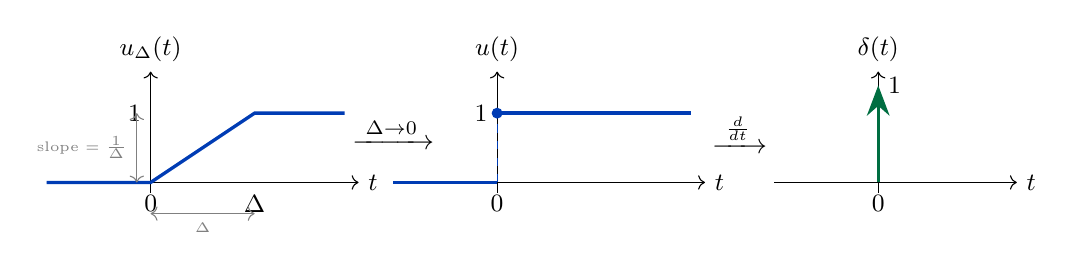
\begin{tikzpicture}[scale=0.88]
  \begin{scope}[xshift=0cm]
    \draw[->](-1.5,0)--(3.0,0) node[right]{\small$t$};
    \draw[->](0,-0.15)--(0,1.6) node[above]{\small$u_\Delta(t)$};
    \draw[myblue,very thick](-1.5,0)--(0,0)--(1.5,1)--(2.8,1);
    \node[below,font=\small] at(0,-0.05){$0$};
    \node[below,font=\small] at(1.5,-0.05){$\Delta$};
    \node[left,font=\small] at(0,1){$1$};
    \draw[<->,gray,thin](-0.2,0)--(-0.2,1) node[midway,left,font=\tiny]{slope $=\tfrac{1}{\Delta}$};
    \draw[<->,gray,thin](0,-0.45)--(1.5,-0.45) node[midway,below,font=\tiny]{$\Delta$};
  \end{scope}
  \node at(3.5,0.7){$\xrightarrow{\;\Delta\to0\;}$};
  \begin{scope}[xshift=5.0cm]
    \draw[->](-1.5,0)--(3.0,0) node[right]{\small$t$};
    \draw[->](0,-0.15)--(0,1.6) node[above]{\small$u(t)$};
    \draw[myblue,very thick](-1.5,0)--(0,0);
    \draw[myblue,very thick](0,1)--(2.8,1);
    \draw[myblue,dashed](0,0)--(0,1);
    \filldraw[myblue](0,1) circle(2pt);
    \node[below,font=\small] at(0,-0.05){$0$};
    \node[left,font=\small] at(0,1){$1$};
  \end{scope}
  \node at(8.5,0.7){$\xrightarrow{\;\frac{d}{dt}\;}$};
  \begin{scope}[xshift=10.5cm]
    \draw[->](-1.5,0)--(2.0,0) node[right]{\small$t$};
    \draw[->](0,-0.15)--(0,1.6) node[above]{\small$\delta(t)$};
    \draw[-{Stealth[scale=1.3]},very thick,darkgreen](0,0)--(0,1.4);
    \node[below,font=\small] at(0,-0.05){$0$};
    \node[right,font=\small] at(0,1.4){$1$};
  \end{scope}
\end{tikzpicture}
\end{center}
\end{derivbox}

\begin{chainbox}
\textbf{Complete Signal Chain (Integration and Differentiation):}
\[
  \delta(t) \;\xrightarrow{\;\int\;}\; u(t) \;\xrightarrow{\;\int\;}\; r(t) \;\xrightarrow{\;\int\;}\; P(t)
  \qquad\qquad
  P(t) \;\xrightarrow{\;\frac{d}{dt}\;}\; r(t) \;\xrightarrow{\;\frac{d}{dt}\;}\; u(t) \;\xrightarrow{\;\frac{d}{dt}\;}\; \delta(t)
\]
\[
  \iint\delta(t)\,dt^2 = r(t) \qquad\qquad \frac{d^2}{dt^2}r(t)=\delta(t) \qquad\qquad \frac{d^3}{dt^3}P(t)=\delta(t)
\]
\end{chainbox}

%% ══════════════════════════════════════════════════════════════════════════════
\section{5.\ Unit Ramp Signal}
%% ══════════════════════════════════════════════════════════════════════════════

\begin{defbox}
The \textbf{unit ramp signal} is defined as:
\[
  r(t) = \begin{cases} 0 & t < 0 \\ t & t \geq 0 \end{cases}
  \qquad\Leftrightarrow\qquad r(t) = t\,u(t)
\]
It is zero for all negative time and then rises with slope (gradient) of $1$ for $t \geq 0$,
passing through the origin at a $45^\circ$ angle. The slope of 1 means: for every 1 second increase in $t$, the amplitude increases by 1 unit.
\end{defbox}

\subsection*{Graph and Variants}

\begin{center}
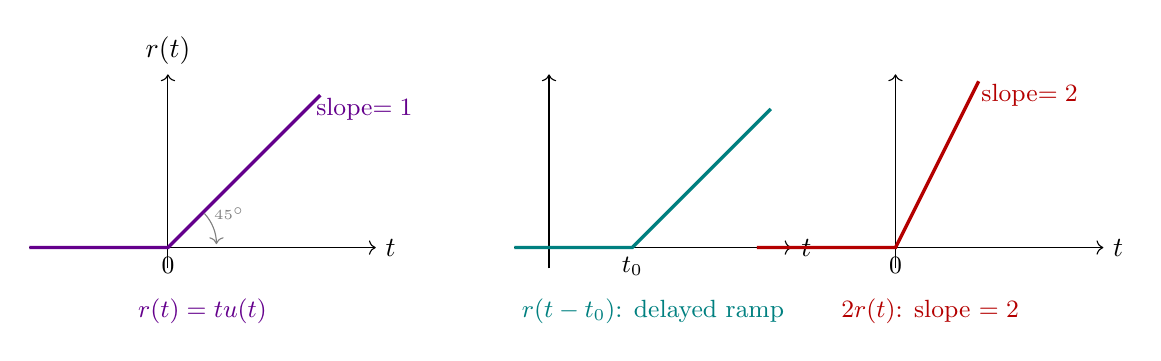
\begin{tikzpicture}[scale=0.88]
  % r(t)
  \begin{scope}[xshift=0cm]
    \draw[->](-2,0)--(3.0,0) node[right]{$t$};
    \draw[->](0,-0.3)--(0,2.5) node[above]{$r(t)$};
    \draw[mypurple,very thick](-2,0)--(0,0)--(2.2,2.2);
    \node[below,font=\small] at(0,0){$0$};
    \node[right,font=\small,mypurple] at(2.0,2.0){slope$=1$};
    \draw[<-,gray,thin] (0.7,0.05) arc(0:43:0.65) node[right,font=\tiny,gray]{$45^\circ$};
    \node[below,font=\small,mypurple] at (0.5,-0.6){$r(t) = tu(t)$};
  \end{scope}
  % r(t-t0)
  \begin{scope}[xshift=5.5cm]
    \draw[->](-0.5,0)--(3.5,0) node[right]{$t$};
    \draw[->](0,-0.3)--(0,2.5) node[above]{};
    \draw[teal,very thick](-0.5,0)--(1.2,0)--(3.2,2.0);
    \node[below,font=\small] at(1.2,0){$t_0$};
    \node[below,font=\small,teal] at(1.5,-0.6){$r(t-t_0)$: delayed ramp};
  \end{scope}
  % 2r(t)
  \begin{scope}[xshift=10.5cm]
    \draw[->](-2,0)--(3.0,0) node[right]{$t$};
    \draw[->](0,-0.3)--(0,2.5) node[above]{};
    \draw[myred,very thick](-2,0)--(0,0)--(1.2,2.4);
    \node[below,font=\small] at(0,0){$0$};
    \node[right,font=\small,myred] at(1.1,2.2){slope$=2$};
    \node[below,font=\small,myred] at (0.5,-0.6){$2r(t)$: slope $=2$};
  \end{scope}
\end{tikzpicture}
\end{center}

\subsection*{Properties of the Unit Ramp Signal}

\begin{propbox}
\textbf{P1 --- Integral Relation:}
\[
  r(t) = \Intt u(\tau)\,d\tau = \int_0^t 1\,d\tau = t \quad (t \geq 0)
\]
So: $u(t)\xrightarrow{\int} r(t)$ and $r(t)\xrightarrow{\frac{d}{dt}} u(t)$.

\medskip
\textbf{P2 --- Relation to step and impulse:}
\[
  \frac{d\,r(t)}{dt} = u(t) \qquad \frac{d^2 r(t)}{dt^2} = \delta(t)
\]

\medskip
\textbf{P3 --- Symmetry:}
$r(t) \neq r(-t)$ (not even) and $r(t) \neq -r(-t)$ (not odd) $\Rightarrow$ \textbf{neither even nor odd}.

Note: $r(-t)=(-t)u(-t)=-tu(-t)=-r_{\rm neg}(t)$, which is a ramp going downward for $t<0$.

\medskip
\textbf{P4 --- Energy and Power:}
\[
  P = \lim_{T\to\infty}\frac{1}{2T}\int_0^T t^2\,dt = \lim_{T\to\infty}\frac{1}{2T}\cdot\frac{T^3}{3} = \lim_{T\to\infty}\frac{T^2}{6} = \infty
\]
\[
  E = \int_0^\infty t^2\,dt = \left.\frac{t^3}{3}\right|_0^\infty = \infty
\]
$E = \infty$, $P = \infty$ $\Rightarrow$ \textbf{NENP signal}

\medskip
\textbf{P5 --- Alternate form using step:}
$r(t) = t\,u(t)$. Any ramp of slope $m$ starting at $t=t_0$ can be written as $m(t-t_0)u(t-t_0)$.
\end{propbox}

\begin{exbox}
\textbf{Constructing ramp from steps:}
A triangular pulse can be constructed:
$x(t)=r(t)-r(t-1)-r(t-2)+r(t-3)$ (a triangle peaking at $t=1$, returning to $0$ at $t=3$)

\textbf{Constructing using step:}
Signal ``starts at 0, ramps up to slope 2 from $t=1$ to $t=4$, then stays constant at 6'':
$x(t)=2(t-1)u(t-1)-2(t-4)u(t-4)$
\end{exbox}

%% ══════════════════════════════════════════════════════════════════════════════
\section{6.\ Unit Parabolic Signal}
%% ══════════════════════════════════════════════════════════════════════════════

\begin{defbox}
The \textbf{unit parabolic signal} (also called the \textbf{acceleration signal}) is defined as:
\[
  P(t) = \begin{cases} 0 & t < 0 \\ \dfrac{t^2}{2} & t \geq 0 \end{cases}
  \qquad\Leftrightarrow\qquad P(t) = \frac{t^2}{2}\,u(t)
\]
It is the integral of the ramp. Note: $2P(t)=t^2$ is a standard upward-opening parabola ($y=x^2$).
Parabola geometry: $t^2 = 2\cdot(2P)$, so in the form $x^2=4ay$, we have $4a=2 \Rightarrow a=\tfrac{1}{2}$.
\end{defbox}

\begin{center}
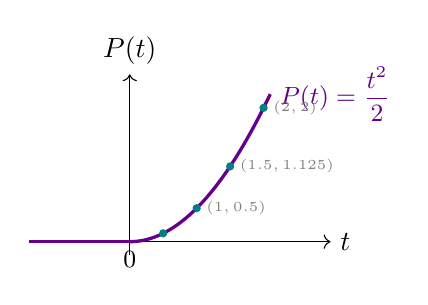
\begin{tikzpicture}[scale=0.85]
  \draw[->](-1.5,0)--(3.0,0) node[right]{$t$};
  \draw[->](0,-0.2)--(0,2.5) node[above]{$P(t)$};
  \draw[mypurple,very thick,domain=0:2.1,samples=60] plot(\x,{0.5*\x*\x});
  \draw[mypurple,very thick](-1.5,0)--(0,0);
  % labels
  \node[below,font=\small] at(0,0){$0$};
  \node[right,font=\small,mypurple] at(2.1,2.2){$P(t)=\dfrac{t^2}{2}$};
  % draw points
  \foreach \x in {0.5,1.0,1.5,2.0}{
    \filldraw[teal] (\x,{0.5*\x*\x}) circle(1.5pt);
  }
  \node[right,font=\tiny,gray] at(1.0,0.5){$(1, 0.5)$};
  \node[right,font=\tiny,gray] at(1.5,1.125){$(1.5, 1.125)$};
  \node[right,font=\tiny,gray] at(2.0,2.0){$(2, 2)$};
\end{tikzpicture}
\end{center}

\begin{propbox}
\textbf{P1 --- Integral Chain:}
\[
  P(t) = \Intt r(\tau)\,d\tau = \int_0^t \tau\,d\tau = \frac{t^2}{2} \quad (t\geq0)
  \qquad\Rightarrow\qquad \frac{d\,P(t)}{dt} = r(t)
\]

\textbf{P2 --- Higher-order derivatives:}
\[
  \frac{d\,P(t)}{dt}=r(t),\quad \frac{d^2P(t)}{dt^2}=u(t),\quad \frac{d^3P(t)}{dt^3}=\delta(t)
\]

\textbf{P3 --- Symmetry:} $P(-t)=P(t)$? No, $P(-t)=\tfrac{(-t)^2}{2}u(-t)=\tfrac{t^2}{2}u(-t)\neq P(t)=\tfrac{t^2}{2}u(t)$\\
$\Rightarrow$ \textbf{Neither even nor odd}

\textbf{P4 --- Energy \& Power:} $E=\infty$, $P=\infty$ $\Rightarrow$ \textbf{NENP signal}
\end{propbox}

\subsection*{Complete Signal Chain Diagram}

\begin{center}
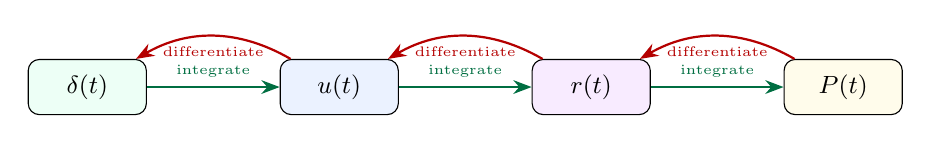
\begin{tikzpicture}[node distance=3.2cm, font=\small]
  \node[draw,rounded corners,fill=lightbg,minimum width=1.5cm,minimum height=0.7cm] (d) at (0,0) {$\delta(t)$};
  \node[draw,rounded corners,fill=stepbg,minimum width=1.5cm,minimum height=0.7cm] (u) at (3.2,0) {$u(t)$};
  \node[draw,rounded corners,fill=rampbg,minimum width=1.5cm,minimum height=0.7cm] (r) at (6.4,0) {$r(t)$};
  \node[draw,rounded corners,fill=expbg,minimum width=1.5cm,minimum height=0.7cm] (p) at (9.6,0) {$P(t)$};
  \draw[-{Stealth},darkgreen,thick] (d) -- node[above,font=\tiny]{integrate} (u);
  \draw[-{Stealth},darkgreen,thick] (u) -- node[above,font=\tiny]{integrate} (r);
  \draw[-{Stealth},darkgreen,thick] (r) -- node[above,font=\tiny]{integrate} (p);
  \draw[-{Stealth},myred,thick] (u) to[bend right=30] node[below,font=\tiny]{differentiate} (d);
  \draw[-{Stealth},myred,thick] (r) to[bend right=30] node[below,font=\tiny]{differentiate} (u);
  \draw[-{Stealth},myred,thick] (p) to[bend right=30] node[below,font=\tiny]{differentiate} (r);
\end{tikzpicture}
\end{center}

%% ══════════════════════════════════════════════════════════════════════════════
\section{7.\ Signum Function (Sign Function)}
%% ══════════════════════════════════════════════════════════════════════════════

\begin{defbox}
The \textbf{signum function} (from Latin \textit{signum} $=$ sign) is defined as:
\[
  \text{sgn}(t) = \begin{cases} -1 & t < 0 \\ 0 & t = 0 \\ +1 & t > 0 \end{cases}
\]
It extracts the \textbf{sign} (polarity) of its argument. Alternative representations:
\[
  \text{sgn}(t) = \frac{|t|}{t} \quad (t \neq 0) \qquad\text{or}\qquad \text{sgn}(t)=2u(t)-1 \quad(t\neq0)
\]
\end{defbox}

\begin{center}
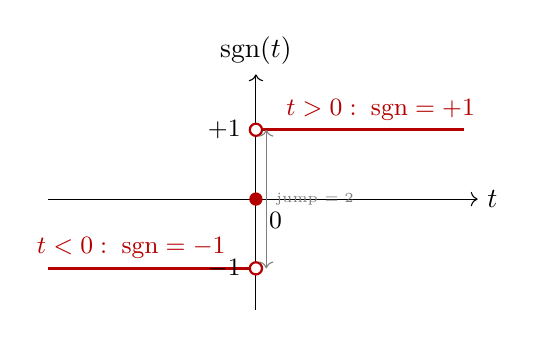
\begin{tikzpicture}[scale=0.88]
  \draw[->](-3.0,0)--(3.2,0) node[right]{$t$};
  \draw[->](0,-1.6)--(0,1.8) node[above]{$\text{sgn}(t)$};
  % horizontal lines
  \draw[myred,very thick](-3.0,-1.0)--(0,-1.0);
  \draw[myred,very thick](0,1.0)--(3.0,1.0);
  % open circles at discontinuity
  \filldraw[white,draw=myred,thick](0,-1.0) circle(2.5pt);
  \filldraw[white,draw=myred,thick](0, 1.0) circle(2.5pt);
  % filled circle at origin
  \filldraw[myred](0,0) circle(2.5pt);
  % labels
  \node[left,font=\small] at(-0.08,1.0){$+1$};
  \node[left,font=\small] at(-0.08,-1.0){$-1$};
  \node[below right,font=\small] at(0.05,-0.05){$0$};
  % region labels
  \node[font=\small,myred,above] at(-1.8,-1.0){$t<0:\;\text{sgn}=-1$};
  \node[font=\small,myred,above] at(1.8, 1.0){$t>0:\;\text{sgn}=+1$};
  % jump arrow
  \draw[<->,gray,thin](0.15,-1.0)--(0.15,1.0) node[midway,right,font=\tiny,gray]{jump $=2$};
\end{tikzpicture}
\end{center}

\begin{propbox}
\textbf{P1 --- Relation to Unit Step:}
\[
  1 + \text{sgn}(t) = 2\,u(t) \qquad\Rightarrow\qquad \boxed{\text{sgn}(t) = 2u(t)-1}
\]
\textit{Verification:} For $t>0$: $1+1=2=2(1)$\checkmark; For $t<0$: $1+(-1)=0=2(0)$\checkmark.

\medskip
\textbf{P2 --- Derivative (relation to impulse):}
\[
  \frac{d}{dt}\text{sgn}(t) = 2\,\delta(t)
\]
Derived by differentiating both sides of $1+\text{sgn}(t)=2u(t)$:
LHS gives $\tfrac{d\,\text{sgn}}{dt}$; RHS gives $2\delta(t)$.

\medskip
\textbf{P3 --- Symmetry:}
$\text{sgn}(-t) = -\text{sgn}(t)$ $\Rightarrow$ \textbf{odd function} (antisymmetric about origin)

\medskip
\textbf{P4 --- Relation to absolute value:}
\[
  \frac{d|t|}{dt} = \text{sgn}(t), \quad t\neq0 \qquad\text{and}\qquad |t| = t\cdot\text{sgn}(t)
\]

\medskip
\textbf{P5 --- Energy and Power:}
\[
  P = \lim_{T\to\infty}\frac{1}{2T}\int_{-T}^{T}|\text{sgn}(t)|^2\,dt = \lim_{T\to\infty}\frac{1}{2T}\cdot 2T = 1
\]
$E=\infty$, $P=1$ (finite) $\Rightarrow$ \textbf{Power signal}.

\medskip
\textbf{P6 --- Numerical Examples:}
$\text{sgn}(-3) = \tfrac{|-3|}{-3} = \tfrac{3}{-3} = -1$; \quad
$\text{sgn}(7) = 1$; \quad
$\text{sgn}(0) = 0$; \quad
$\text{sgn}(\pi-3) = \text{sgn}(+0.14) = +1$ (since $\pi\approx3.14>3$)
\end{propbox}

\begin{exbox}
\textbf{Express the signum in terms of step and vice versa:}

From $\text{sgn}(t)=2u(t)-1$:
\[
  u(t) = \frac{1+\text{sgn}(t)}{2}
\]

\textbf{Relation diagram:}
\[
  \delta(t)\xrightarrow{\int} u(t)\xleftrightarrow{\;\text{sgn}(t)=2u(t)-1\;}\text{sgn}(t)\xrightarrow{\;\frac{d}{dt}\;} 2\delta(t)
\]

\textbf{Sketch $y(t) = \text{sgn}(t)\cdot u(t)$:}
For $t>0$: $1\times1=1$; for $t<0$: $(-1)\times 0=0$; at $t=0$: $0\times1=0$.\\
$\Rightarrow$ $y(t)=u(t)$ (exactly the unit step)! So $\text{sgn}(t)\cdot u(t)=u(t)$.
\end{exbox}

%% ══════════════════════════════════════════════════════════════════════════════
\section{8.\ Unit Rectangular Pulse (Gate Function)}
%% ══════════════════════════════════════════════════════════════════════════════

\begin{defbox}
The \textbf{unit rectangular pulse} (also called the \textbf{gate function} or \textbf{rect function}) is a pulse symmetric about the origin with \textbf{unit area}:
\[
  \text{rect}(t) = \begin{cases} 0 & |t| > \tfrac{a}{2} \\ \dfrac{1}{a} & |t| \leq \tfrac{a}{2} \end{cases}
  \qquad\text{Width}=a, \quad\text{Height}=\tfrac{1}{a}, \quad\text{Area}=a\times\tfrac{1}{a}=1
\]
When $a=1$: $\text{rect}(t) = 1$ for $|t|\leq\tfrac{1}{2}$, which is the \textbf{standard unit rectangular pulse}.
\end{defbox}

\begin{center}
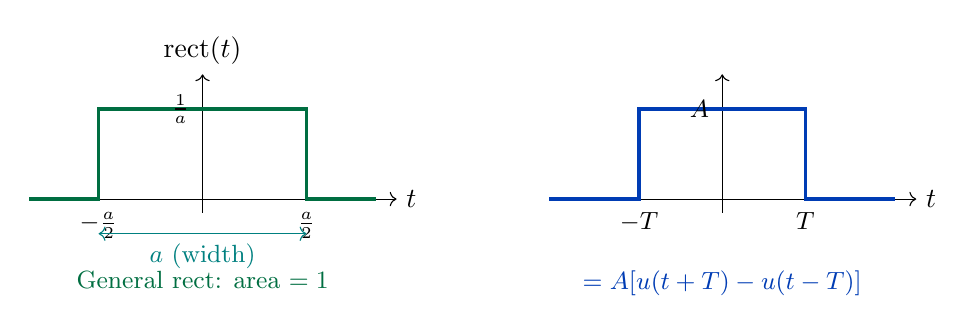
\begin{tikzpicture}[scale=0.88]
  % Standard rect
  \begin{scope}[xshift=0cm]
    \draw[->](-2.5,0)--(2.8,0) node[right]{$t$};
    \draw[->](0,-0.2)--(0,1.8) node[above]{rect$(t)$};
    \draw[darkgreen,very thick](-2.5,0)--(-1.5,0)--(-1.5,1.3)--(1.5,1.3)--(1.5,0)--(2.5,0);
    \node[below,font=\small] at(-1.5,-0.05){$-\frac{a}{2}$};
    \node[below,font=\small] at(1.5,-0.05){$\frac{a}{2}$};
    \node[left,font=\small] at(-0.05,1.3){$\frac{1}{a}$};
    \draw[<->,teal,thin](-1.5,-0.5)--(1.5,-0.5) node[midway,below,font=\small]{$a$ (width)};
    \node[below,font=\small,darkgreen] at(0,-0.9){General rect: area $=1$};
  \end{scope}
  % Rect as step difference
  \begin{scope}[xshift=7.5cm]
    \draw[->](-2.5,0)--(2.8,0) node[right]{$t$};
    \draw[->](0,-0.2)--(0,1.8) node[above]{};
    \draw[myblue,very thick](-2.5,0)--(-1.2,0)--(-1.2,1.3)--(1.2,1.3)--(1.2,0)--(2.5,0);
    \node[below,font=\small] at(-1.2,-0.05){$-T$};
    \node[below,font=\small] at(1.2,-0.05){$T$};
    \node[left,font=\small] at(-0.05,1.3){$A$};
    \node[below,font=\small,myblue] at(0,-0.9){$= A[u(t+T)-u(t-T)]$};
  \end{scope}
\end{tikzpicture}
\end{center}

\begin{propbox}
\textbf{P1 --- Even Symmetry:}
$\text{rect}(-t) = \text{rect}(t)$ (symmetric about $t=0$) $\Rightarrow$ \textbf{even function}

\medskip
\textbf{P2 --- Expression using Unit Steps:}
\[
  \text{rect}(t/a) = u\!\bigl(t+\tfrac{a}{2}\bigr) - u\!\bigl(t-\tfrac{a}{2}\bigr) \qquad \text{(difference of two steps)}
\]
This is extremely useful for constructing piecewise signals.

\medskip
\textbf{P3 --- Energy:}
\[
  E = \int_{-a/2}^{a/2} \left(\frac{1}{a}\right)^2 dt = \frac{1}{a^2}\cdot a = \frac{1}{a}
\]
$E=\tfrac{1}{a}$ is finite $\Rightarrow$ \textbf{Energy signal} (provided $a>0$ and finite).

\medskip
\textbf{P4 --- Power:}
\[
  P = \lim_{T\to\infty}\frac{1}{2T}\int_{-a/2}^{a/2}\frac{1}{a^2}\,dt = \lim_{T\to\infty}\frac{a\cdot(1/a^2)}{2T} = \lim_{T\to\infty}\frac{1}{2aT} = 0
\]
$P=0$ (consistent with being an energy signal; energy signals always have $P=0$).

\medskip
\textbf{P5 --- Limit gives impulse:}
As $a\to0$: width $\to0$, height $=1/a\to\infty$, area stays $=1$ $\Rightarrow \text{rect}(t/a)\to\delta(t)$.

\medskip
\textbf{P6 --- Fourier Transform:}
\[
  \text{rect}(t/a) \xrightarrow{\mathcal{F}} a\,\text{sinc}(af) \qquad (\text{rectangular pulse} \leftrightarrow \text{sinc spectrum})
\]
\end{propbox}

\begin{exbox}
\textbf{Constructing a trapezoidal pulse:}
$x(t) = r(t+2)-r(t+1)-r(t-1)+r(t-2)$

\textbf{Pulse train (periodic rect):} $\sum_{n=-\infty}^{\infty}\text{rect}\bigl(\tfrac{t-nT_0}{\tau}\bigr)$ --- duty cycle $= \tau/T_0$.

\textbf{Duty cycle of a pulse:} $D=\tau/T_0$ where $\tau=$ pulse width, $T_0=$ period.
\end{exbox}

%% ══════════════════════════════════════════════════════════════════════════════
\section{9.\ Unit Triangular Function}
%% ══════════════════════════════════════════════════════════════════════════════

\begin{defbox}
The \textbf{unit triangular function} is a piecewise linear signal that rises linearly from 0 to a peak of 1 at $t=0$, then falls linearly back to 0:
\[
  \text{tri}(t) = \begin{cases} t+1 & -1\leq t\leq 0 \\ -t+1 & 0\leq t\leq 1 \\ 0 & |t|>1 \end{cases}
  \qquad\text{Area}=\tfrac{1}{2}\times\text{base}\times\text{height}=\tfrac{1}{2}\times 2\times 1=1
\]
\end{defbox}

\begin{center}
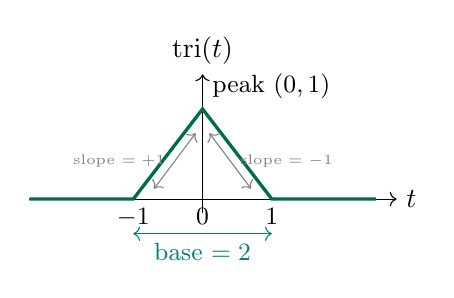
\begin{tikzpicture}[scale=0.88]
  \draw[->](-2.5,0)--(2.8,0) node[right]{$t$};
  \draw[->](0,-0.2)--(0,1.8) node[above]{tri$(t)$};
  \draw[darkgreen,very thick](-2.5,0)--(-1,0)--(0,1.3)--(1,0)--(2.5,0);
  \node[below,font=\small] at(-1,0){$-1$};
  \node[below,font=\small] at(0,0){$0$};
  \node[below,font=\small] at(1,0){$1$};
  \node[above right,font=\small] at(0,1.3){peak $(0,1)$};
  % Slope labels
  \draw[<->,gray,thin] (-0.7,0.15) -- (-0.1,0.95) node[midway,left,font=\tiny,gray]{slope $=+1$};
  \draw[<->,gray,thin] (0.1,0.95) -- (0.7,0.15) node[midway,right,font=\tiny,gray]{slope $=-1$};
  % Area label
  \draw[<->,teal,thin](-1,-0.5)--(1,-0.5) node[midway,below,font=\small]{base $=2$};
\end{tikzpicture}
\end{center}

\begin{propbox}
\textbf{P1 --- Even Symmetry:}
$\text{tri}(-t) = \text{tri}(t)$ $\Rightarrow$ \textbf{even function} (symmetric about $t=0$)

\medskip
\textbf{P2 --- Expression using rects (convolution):}
$\text{tri}(t) = \text{rect}(t) * \text{rect}(t)$ (convolution of two rect pulses).
This is why the triangular pulse has a \textbf{sinc}$^2$ Fourier transform.

\medskip
\textbf{P3 --- Expression using ramps:}
\[
  \text{tri}(t) = r(t+1) - 2r(t) + r(t-1) \qquad (\text{second difference of ramps})
\]

\medskip
\textbf{P4 --- Energy:}
\[
  E = \int_{-1}^{0}(t+1)^2\,dt + \int_{0}^{1}(1-t)^2\,dt
    = \left[\frac{(t+1)^3}{3}\right]_{-1}^{0}+\left[-\frac{(1-t)^3}{3}\right]_{0}^{1}
    = \frac{1}{3}+\frac{1}{3} = \frac{2}{3}
\]
$E=\tfrac{2}{3}$ (finite) $\Rightarrow$ \textbf{Energy signal}

\medskip
\textbf{P5 --- Power:} $P=0$ (since $E$ is finite and signal is finite duration $\Rightarrow$ zero average power).

\medskip
\textbf{P6 --- Fourier Transform:}
\[
  \text{tri}(t) \xrightarrow{\mathcal{F}} \text{sinc}^2(f) \qquad (\text{triangle}\leftrightarrow\text{sinc}^2)
\]
\end{propbox}

%% ══════════════════════════════════════════════════════════════════════════════
\section{10.\ Sinc Function (Cardinal Sine)}
%% ══════════════════════════════════════════════════════════════════════════════

\begin{defbox}
There are two common definitions of the sinc function:

\textbf{Unnormalized sinc:}
\[
  \text{sinc}(t) = \begin{cases} 1 & t=0 \\ \dfrac{\sin t}{t} & t\neq0 \end{cases}
\]
Zeros at $t = \pm\pi, \pm2\pi, \pm3\pi, \ldots$ (i.e., nonzero multiples of $\pi$)

\medskip
\textbf{Normalized sinc} (used in DSP and communications):
\[
  \text{sinc}(t) = \begin{cases} 1 & t=0 \\ \dfrac{\sin(\pi t)}{\pi t} & t\neq0 \end{cases}
\]
Zeros at $t = \pm1, \pm2, \pm3, \ldots$ (all nonzero integers). \quad\textit{Value at $t=0$ is 1 for both forms (by L'Hôpital's rule).}
\end{defbox}

\begin{center}
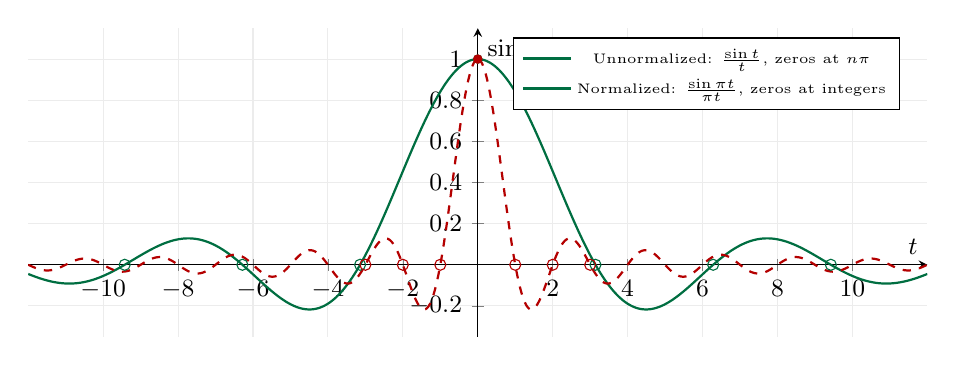
\begin{tikzpicture}
  \begin{axis}[
    width=13cm, height=5.5cm,
    xlabel={$t$}, ylabel={sinc$(t)$},
    xmin=-12, xmax=12, ymin=-0.35, ymax=1.15,
    axis lines=center,
    tick label style={font=\small},
    label style={font=\small},
    samples=400,
    grid=both, grid style={gray!15},
    xtick={-10,-8,-6,-4,-2,0,2,4,6,8,10},
    ytick={-0.2,0,0.2,0.4,0.6,0.8,1.0},
    legend pos=north east,
    legend style={font=\tiny},
  ]
    \addplot[darkgreen,thick,domain=-12:-0.01]{sin(deg(x))/x};
    \addplot[darkgreen,thick,domain=0.01:12]{sin(deg(x))/x};
    \addplot[darkgreen,only marks,mark=*,mark size=1.5pt] coordinates{(0,1)};
    \addlegendentry{Unnormalized: $\frac{\sin t}{t}$, zeros at $n\pi$};
    \addplot[myred,dashed,thick,domain=-12:-0.01]{sin(deg(pi*x))/(pi*x)};
    \addplot[myred,dashed,thick,domain=0.01:12]{sin(deg(pi*x))/(pi*x)};
    \addplot[myred,only marks,mark=*,mark size=1.5pt] coordinates{(0,1)};
    \addlegendentry{Normalized: $\frac{\sin\pi t}{\pi t}$, zeros at integers};
    % Mark zeros of unnormalized
    \foreach \z in {-3.14159,-6.28318,-9.42478,3.14159,6.28318,9.42478}{
      \addplot[darkgreen,only marks,mark=o,mark size=2pt] coordinates{(\z,0)};
    }
    % Mark zeros of normalized
    \foreach \z in {-3,-2,-1,1,2,3}{
      \addplot[myred,only marks,mark=o,mark size=2pt] coordinates{(\z,0)};
    }
  \end{axis}
\end{tikzpicture}
\end{center}

\begin{propbox}
\textbf{P1 --- Value at origin:} By L'Hôpital's rule: $\lim_{t\to0}\frac{\sin t}{t}=1$ (unnorm.) and $\lim_{t\to0}\frac{\sin\pi t}{\pi t}=1$ (norm.)

\medskip
\textbf{P2 --- Even symmetry:} $\text{sinc}(-t) = \text{sinc}(t)$ $\Rightarrow$ \textbf{even function}

\medskip
\textbf{P3 --- Zeros:}
\begin{itemize}
  \item Unnormalized: at $t = \pm n\pi$ for $n = 1, 2, 3, \ldots$
  \item Normalized: at $t = \pm n$ (all nonzero integers)
\end{itemize}

\medskip
\textbf{P4 --- Decay:} $\text{sinc}(t) \to 0$ as $|t| \to \infty$ (oscillates with decreasing amplitude)

\medskip
\textbf{P5 --- Energy (unnormalized):}
\[
  E = \Int \left|\frac{\sin t}{t}\right|^2 dt = \pi
\]
Finite energy $\Rightarrow$ \textbf{Energy signal}.

\medskip
\textbf{P6 --- Energy for scaled sinc:}
$E\bigl[\text{sinc}(at)\bigr] = \dfrac{\pi}{a}$ \quad (e.g., $\text{sinc}(\pi t) \Rightarrow E = \dfrac{\pi}{\pi} = 1$)

\medskip
\textbf{P7 --- Key integral:}
\[
  \Int \frac{\sin t}{t}\,dt = \pi \qquad (\text{Dirichlet integral})
\]

\medskip
\textbf{P8 --- Fourier Transform relationship:}
\[
  \text{rect}(t) \xrightarrow{\mathcal{F}} \text{sinc}(f) \qquad\text{and}\qquad \text{sinc}(t) \xrightarrow{\mathcal{F}} \text{rect}(f)
\]
This duality is fundamental in DSP and communications theory.

\medskip
\textbf{P9 --- Power:} $P = 0$ (since $E$ is finite, $P = E / \infty = 0$). $\Rightarrow$ \textbf{Energy signal, not power signal}.

\medskip
\textbf{P10 --- Orthogonality:} Normalized sinc functions shifted by integers are \textbf{orthogonal}:
\[
  \Int \text{sinc}(t-m)\,\text{sinc}(t-n)\,dt = \delta_{mn} \quad (\text{Kronecker delta})
\]
This is the basis of ideal Nyquist interpolation in sampling theory.
\end{propbox}

\begin{notebox}
\textbf{Why sinc appears everywhere in signals and systems:}
\begin{itemize}
  \item The Fourier Transform of a rectangular window is a sinc --- so any finite-duration observation introduces sinc-shaped spectral leakage.
  \item In ideal (Nyquist) reconstruction: $x(t) = \sum_{n=-\infty}^{\infty} x[n]\,\text{sinc}\!\bigl(\tfrac{t-nT_s}{T_s}\bigr)$
  \item The sinc is the \emph{ideal lowpass filter} impulse response --- it passes all frequencies below $W$ and blocks all above.
\end{itemize}
\end{notebox}

%% ══════════════════════════════════════════════════════════════════════════════
\section{11.\ Exponential Signals (Real and Complex)}
%% ══════════════════════════════════════════════════════════════════════════════

\begin{defbox}
\textbf{General form:} $x(t) = A_0\,e^{\beta t}$ where $\beta \in \mathbb{C}$, $A_0$ is a constant.

\textbf{Complex exponent:} $\beta = \sigma + j\omega$ where $\sigma = \mathrm{Re}(\beta)$ (real part, controls growth/decay) and $\omega = \mathrm{Im}(\beta)$ (imaginary part, controls oscillation frequency).

\textbf{Euler's formula:} $e^{j\theta} = \cos\theta + j\sin\theta$

\textbf{Full expansion:}
\[
  x(t) = A_0\,e^{(\sigma+j\omega)t} = A_0\,e^{\sigma t}\cdot e^{j\omega t} = A_0\,e^{\sigma t}\bigl(\cos\omega t + j\sin\omega t\bigr)
\]
The factor $e^{\sigma t}$ is the \textbf{envelope} (amplitude modulation); $e^{j\omega t}$ is the \textbf{oscillating phasor}.
\end{defbox}

\subsection*{Case I: $\omega = 0$ --- Real Exponential $x(t) = e^{\sigma t}$}

\begin{center}
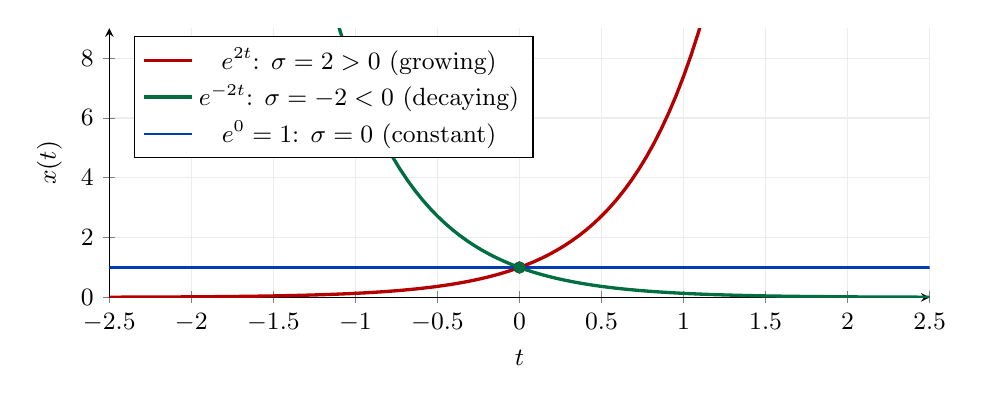
\begin{tikzpicture}
  \begin{axis}[
    width=12cm, height=5cm,
    xlabel={$t$}, ylabel={$x(t)$},
    xmin=-2.5, xmax=2.5, ymin=0, ymax=9,
    axis lines=left,
    tick label style={font=\small},
    label style={font=\small},
    samples=100,
    grid=both, grid style={gray!15},
    legend pos=north west,
    legend style={font=\small},
  ]
    \addplot[myred,very thick,domain=-2.5:2]{exp(2*x)};
    \addlegendentry{$e^{2t}$: $\sigma=2>0$ (growing)};
    \addplot[darkgreen,very thick,domain=-2:2.5]{exp(-2*x)};
    \addlegendentry{$e^{-2t}$: $\sigma=-2<0$ (decaying)};
    \addplot[myblue,thick,domain=-2.5:2.5]{1};
    \addlegendentry{$e^{0} = 1$: $\sigma=0$ (constant)};
    % Mark value at t=0
    \addplot[only marks,mark=*,myred,mark size=2pt] coordinates{(0,1)};
    \addplot[only marks,mark=*,darkgreen,mark size=2pt] coordinates{(0,1)};
  \end{axis}
\end{tikzpicture}
\end{center}

\begin{propbox}
\textbf{Sub-case 1 --- $\sigma > 0$ (Growing exponential):}
\[
  x(t) = e^{\sigma t} \to \infty \quad \text{as} \quad t \to +\infty
\]
Energy: $E=\int_{-\infty}^{\infty}e^{2\sigma t}\,dt=\infty$. Power: $P=\infty$. $\Rightarrow$ \textbf{NENP signal}

\medskip
\textbf{Sub-case 2 --- $\sigma < 0$ (Decaying/Damped exponential):}
\[
  x(t) = e^{-|\sigma| t} \to 0 \quad \text{as} \quad t \to +\infty \quad\text{(converges)}
\]
For the one-sided causal version $x(t)=e^{-at}u(t)$, $a>0$:
\[
  E = \int_0^{\infty} e^{-2at}\,dt = \frac{1}{2a} \quad\text{(finite)} \Rightarrow \textbf{Energy signal}
\]
Time constant $\tau = \dfrac{1}{a}$: the signal decays to $e^{-1}\approx37\%$ of its initial value after time $\tau$.

\medskip
\textbf{Sub-case 3 --- $\sigma = 0$:}
$x(t) = e^0 = 1$ (DC signal --- constant, infinite energy, $P=1$).
\end{propbox}

\subsection*{Case II: $\omega \neq 0$ --- Complex Exponential}

\[
  x(t) = e^{(\sigma+j\omega)t} = e^{\sigma t}(\cos\omega t + j\sin\omega t)
\]

\begin{center}
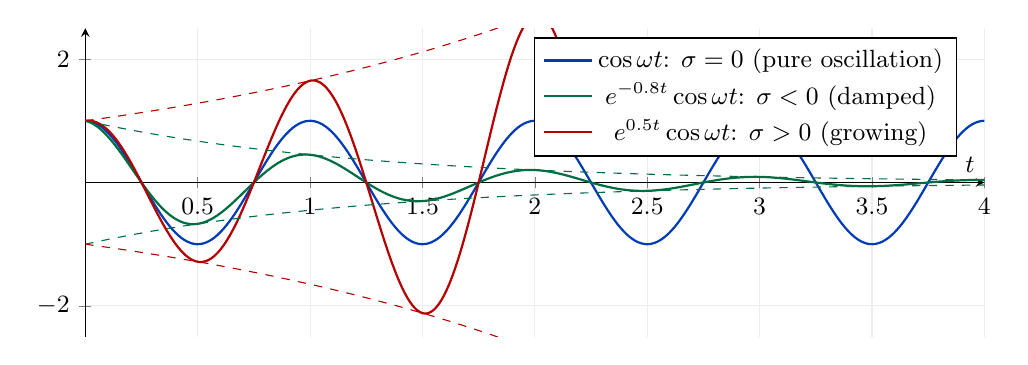
\begin{tikzpicture}
  \begin{axis}[
    width=13cm, height=5.5cm,
    xlabel={$t$}, ylabel={},
    xmin=0, xmax=4, ymin=-2.5, ymax=2.5,
    axis lines=center,
    tick label style={font=\small},
    label style={font=\small},
    samples=300,
    grid=both, grid style={gray!15},
    legend pos=north east,
    legend style={font=\small},
  ]
    % Pure sinusoid (sigma=0)
    \addplot[myblue,thick,domain=0:4]{cos(deg(2*pi*x))};
    \addlegendentry{$\cos\omega t$: $\sigma=0$ (pure oscillation)};
    % Decaying
    \addplot[darkgreen,thick,domain=0:4]{exp(-0.8*x)*cos(deg(2*pi*x))};
    \addlegendentry{$e^{-0.8t}\cos\omega t$: $\sigma<0$ (damped)};
    % Growing
    \addplot[myred,thick,domain=0:2.2]{exp(0.5*x)*cos(deg(2*pi*x))};
    \addlegendentry{$e^{0.5t}\cos\omega t$: $\sigma>0$ (growing)};
    % Envelope curves
    \addplot[darkgreen,dashed,thin,domain=0:4]{exp(-0.8*x)};
    \addplot[darkgreen,dashed,thin,domain=0:4]{-exp(-0.8*x)};
    \addplot[myred,dashed,thin,domain=0:2.2]{exp(0.5*x)};
    \addplot[myred,dashed,thin,domain=0:2.2]{-exp(0.5*x)};
  \end{axis}
\end{tikzpicture}
\end{center}

\begin{propbox}
\textbf{Sub-case 1 --- $\sigma = 0$: Pure Sinusoidal / Phasor}
\[
  x(t) = e^{j\omega t} = \cos\omega t + j\sin\omega t \quad\text{(constant amplitude envelope)}
\]
Real part: $\cos\omega t$ (cosine wave). Imaginary part: $\sin\omega t$ (sine wave).
In 3D: traces a \textbf{helix} along the time axis with constant radius.
$E=\infty$, $P=1$ $\Rightarrow$ \textbf{Power signal}.

\medskip
\textbf{Sub-case 2 --- $\sigma > 0$: Growing Oscillation}
\[
  x(t) = e^{\sigma t}\cos\omega t \quad\text{(amplitude envelope} = e^{\sigma t} \text{expands)}
\]
Amplitude increases exponentially. Both $E$ and $P$ are infinite $\Rightarrow$ \textbf{NENP}.
Represents unstable systems in control theory.

\medskip
\textbf{Sub-case 3 --- $\sigma < 0$: Damped Oscillation}
\[
  x(t) = e^{\sigma t}\cos\omega t \quad\text{(amplitude envelope} = e^{-|\sigma|t} \text{shrinks)}
\]
Amplitude decays exponentially toward zero. For causal version: $E=\dfrac{1}{2|\sigma|}$ (finite)
$\Rightarrow$ \textbf{Energy signal}. Represents stable systems (e.g., RLC circuits, mechanical damping).
\end{propbox}

\subsection*{Summary: All Cases of $x(t) = e^{(\sigma+j\omega)t}$}

\begin{center}
{\small
\begin{tabular}{@{}ccc p{4.5cm} c@{}}
\toprule
$\sigma$ & $\omega$ & Type & Behaviour & Classification \\
\midrule
$>0$ & $0$ & Real growing & Monotone growth to $\infty$ & NENP \\
$<0$ & $0$ & Real decaying & Monotone decay to $0$ & Energy ($E=\tfrac{1}{2|\sigma|}$) \\
$0$ & $0$ & DC constant & Flat line $x=A_0$ & Power ($P=A_0^2$) \\
$0$ & $\neq0$ & Pure sinusoid & Constant-amplitude oscillation & Power ($P=\tfrac{1}{2}$) \\
$>0$ & $\neq0$ & Growing oscillation & Expanding spiral & NENP \\
$<0$ & $\neq0$ & Damped oscillation & Decaying spiral (stable) & Energy \\
\bottomrule
\end{tabular}
}
\end{center}

\begin{exbox}
\textbf{Example 1:} Classify $x(t) = 5e^{-3t}u(t)$.\\
$\sigma=-3<0$, $\omega=0$, causal. $E=\int_0^\infty 25e^{-6t}\,dt=\tfrac{25}{6}$. Finite $\Rightarrow$ \textbf{Energy signal}, $E=\tfrac{25}{6}$.

\medskip
\textbf{Example 2:} Classify $x(t)=e^{j2\pi f_0 t}$.\\
$\sigma=0$, $\omega=2\pi f_0\neq0$. $P=\lim_{T\to\infty}\tfrac{1}{2T}\int_{-T}^{T}|e^{j2\pi f_0t}|^2dt=1$. $\Rightarrow$ \textbf{Power signal}, $P=1$.

\medskip
\textbf{Example 3 (Euler):} Express $\cos\omega_0 t$ and $\sin\omega_0 t$ using complex exponentials:
\[
  \cos\omega_0 t = \frac{e^{j\omega_0 t}+e^{-j\omega_0 t}}{2} \qquad\qquad \sin\omega_0 t = \frac{e^{j\omega_0 t}-e^{-j\omega_0 t}}{2j}
\]

\textbf{Example 4:} Find the time constant of $x(t)=e^{-500t}u(t)$.\\
$a=500$ $\Rightarrow$ $\tau=\tfrac{1}{500}=2\,\mathrm{ms}$. After $5\tau=10\,\mathrm{ms}$ the signal is approximately $0$ (within $1\%$).
\end{exbox}

%% ══════════════════════════════════════════════════════════════════════════════
\section{Quick Reference: Signal Classification Summary}
%% ══════════════════════════════════════════════════════════════════════════════

\begin{center}
{\small
\begin{tabular}{@{}l c c c c c@{}}
\toprule
\textbf{Signal} & \textbf{Even/Odd} & \textbf{Energy $E$} & \textbf{Power $P$} & \textbf{Type} & \textbf{Fourier Transform} \\
\midrule
$\delta(t)$ & Even & $\infty$ & $\infty$ & NENP & $1$ \\
$u(t)$ & Neither & $\infty$ & $1/2$ & Power & $\tfrac{1}{2}\delta(f)+\tfrac{1}{j2\pi f}$ \\
$r(t)=tu(t)$ & Neither & $\infty$ & $\infty$ & NENP & --- \\
$P(t)=\tfrac{t^2}{2}u(t)$ & Neither & $\infty$ & $\infty$ & NENP & --- \\
$\text{sgn}(t)$ & Odd & $\infty$ & $1$ & Power & $\tfrac{1}{j\pi f}$ \\
$\text{rect}(t)$ & Even & $1/a$ & $0$ & Energy & $a\,\text{sinc}(af)$ \\
$\text{tri}(t)$ & Even & $2/3$ & $0$ & Energy & $\text{sinc}^2(f)$ \\
$\text{sinc}(t)$ & Even & $\pi$ & $0$ & Energy & $\text{rect}(f)$ \\
$e^{j\omega_0 t}$ & Neither & $\infty$ & $1$ & Power & $\delta(f-f_0)$ \\
$e^{-at}u(t)$ & Neither & $\tfrac{1}{2a}$ & $0$ & Energy & $\tfrac{1}{a+j2\pi f}$ \\
\bottomrule
\end{tabular}
}
\end{center}

\vspace{6pt}
\begin{center}
{\small\color{gray}
Signals \& Systems $\cdot$ EC002 $\cdot$ Comprehensive Reference Notes (Unit Impulse through Exponential Signals)
}
\end{center}

\end{document}